\documentclass{article}
\usepackage[T1]{fontenc}
\usepackage[utf8]{inputenc}
\usepackage[margin=1in]{geometry}
\usepackage{fancyhdr} 
\usepackage{listings}
\usepackage{algorithm}
\usepackage[noend]{algorithmic}
\usepackage{amsmath, amsthm, amssymb, amsfonts}
\usepackage{graphicx}
\usepackage[dvipsnames]{xcolor}
\usepackage{xy}
\usepackage{url}
\usepackage{parskip}
\usepackage{comment}
\usepackage{setspace}
\usepackage{enumerate}
\usepackage{multirow}
\usepackage{hyperref}
\usepackage{caption}
\usepackage{subcaption}
\usepackage{booktabs}
\usepackage{wrapfig}
\usepackage{times}

\captionsetup[figure]{font={small,it}}

\usepackage[backend=biber,style=numeric,sortcites,maxbibnames=99]{biblatex}
\addbibresource{references.bib}

\newcommand{\HRule}{\rule{\linewidth}{0.5mm}}
\newcommand{\Hrule}{\rule{\linewidth}{0.3mm}}
\newcommand{\classnum}{CS-GY 6313 B}

\makeatletter% since there's an at-sign (@) in the command name
\renewcommand{\@maketitle}{%
  \parindent=0pt% don't indent paragraphs in the title block
  \centering
  {\Large \bfseries\textsc{\@title}}
  \HRule\par%
  \textit{\@author \hfill \classnum}
  \par
}
\makeatother% resets the meaning of the at-sign (@)

\title{Assignment 3: Interactive Visualization}
\author{Sanyukta Tuti}
% \classnum

\begin{document}
  \maketitle % prints the title block
  \thispagestyle{empty}
  % \vspace{-15pt}

\section{Introduction}
\label{sec:sec1}

\maketitle

In this assignment, we created an interactive visualization to explore the trade relationships of the top five trading countries based on total trade value, utilizing the \textbf{Global Commodity Trade Statistics}\cite{dataset} dataset on Kaggle which was referenced from and published by the United Nations Statistics Division on the UNData site. The visualization focuses on the import and export activities of these countries, providing insights into their trade categories and volume. The goal is to allow users to interactively examine trade flows and gain a deeper understanding of global trade dynamics. The goal is to answer the following questions:

\begin{enumerate}
    \item \textit{"Which countries are the top traders in terms of total trade value?"}
    \item \textit{"How do the import and export activities of these countries vary across different commodity categories?"}
    \item \textit{"What insights can we derive about trade flow trends among these top trading countries?"}
\end{enumerate}


\section{Visual Insights into Import and Export Activities of the Top Trading Countries (1988-2016)}

\begin{figure}[ht] 
    \centering
    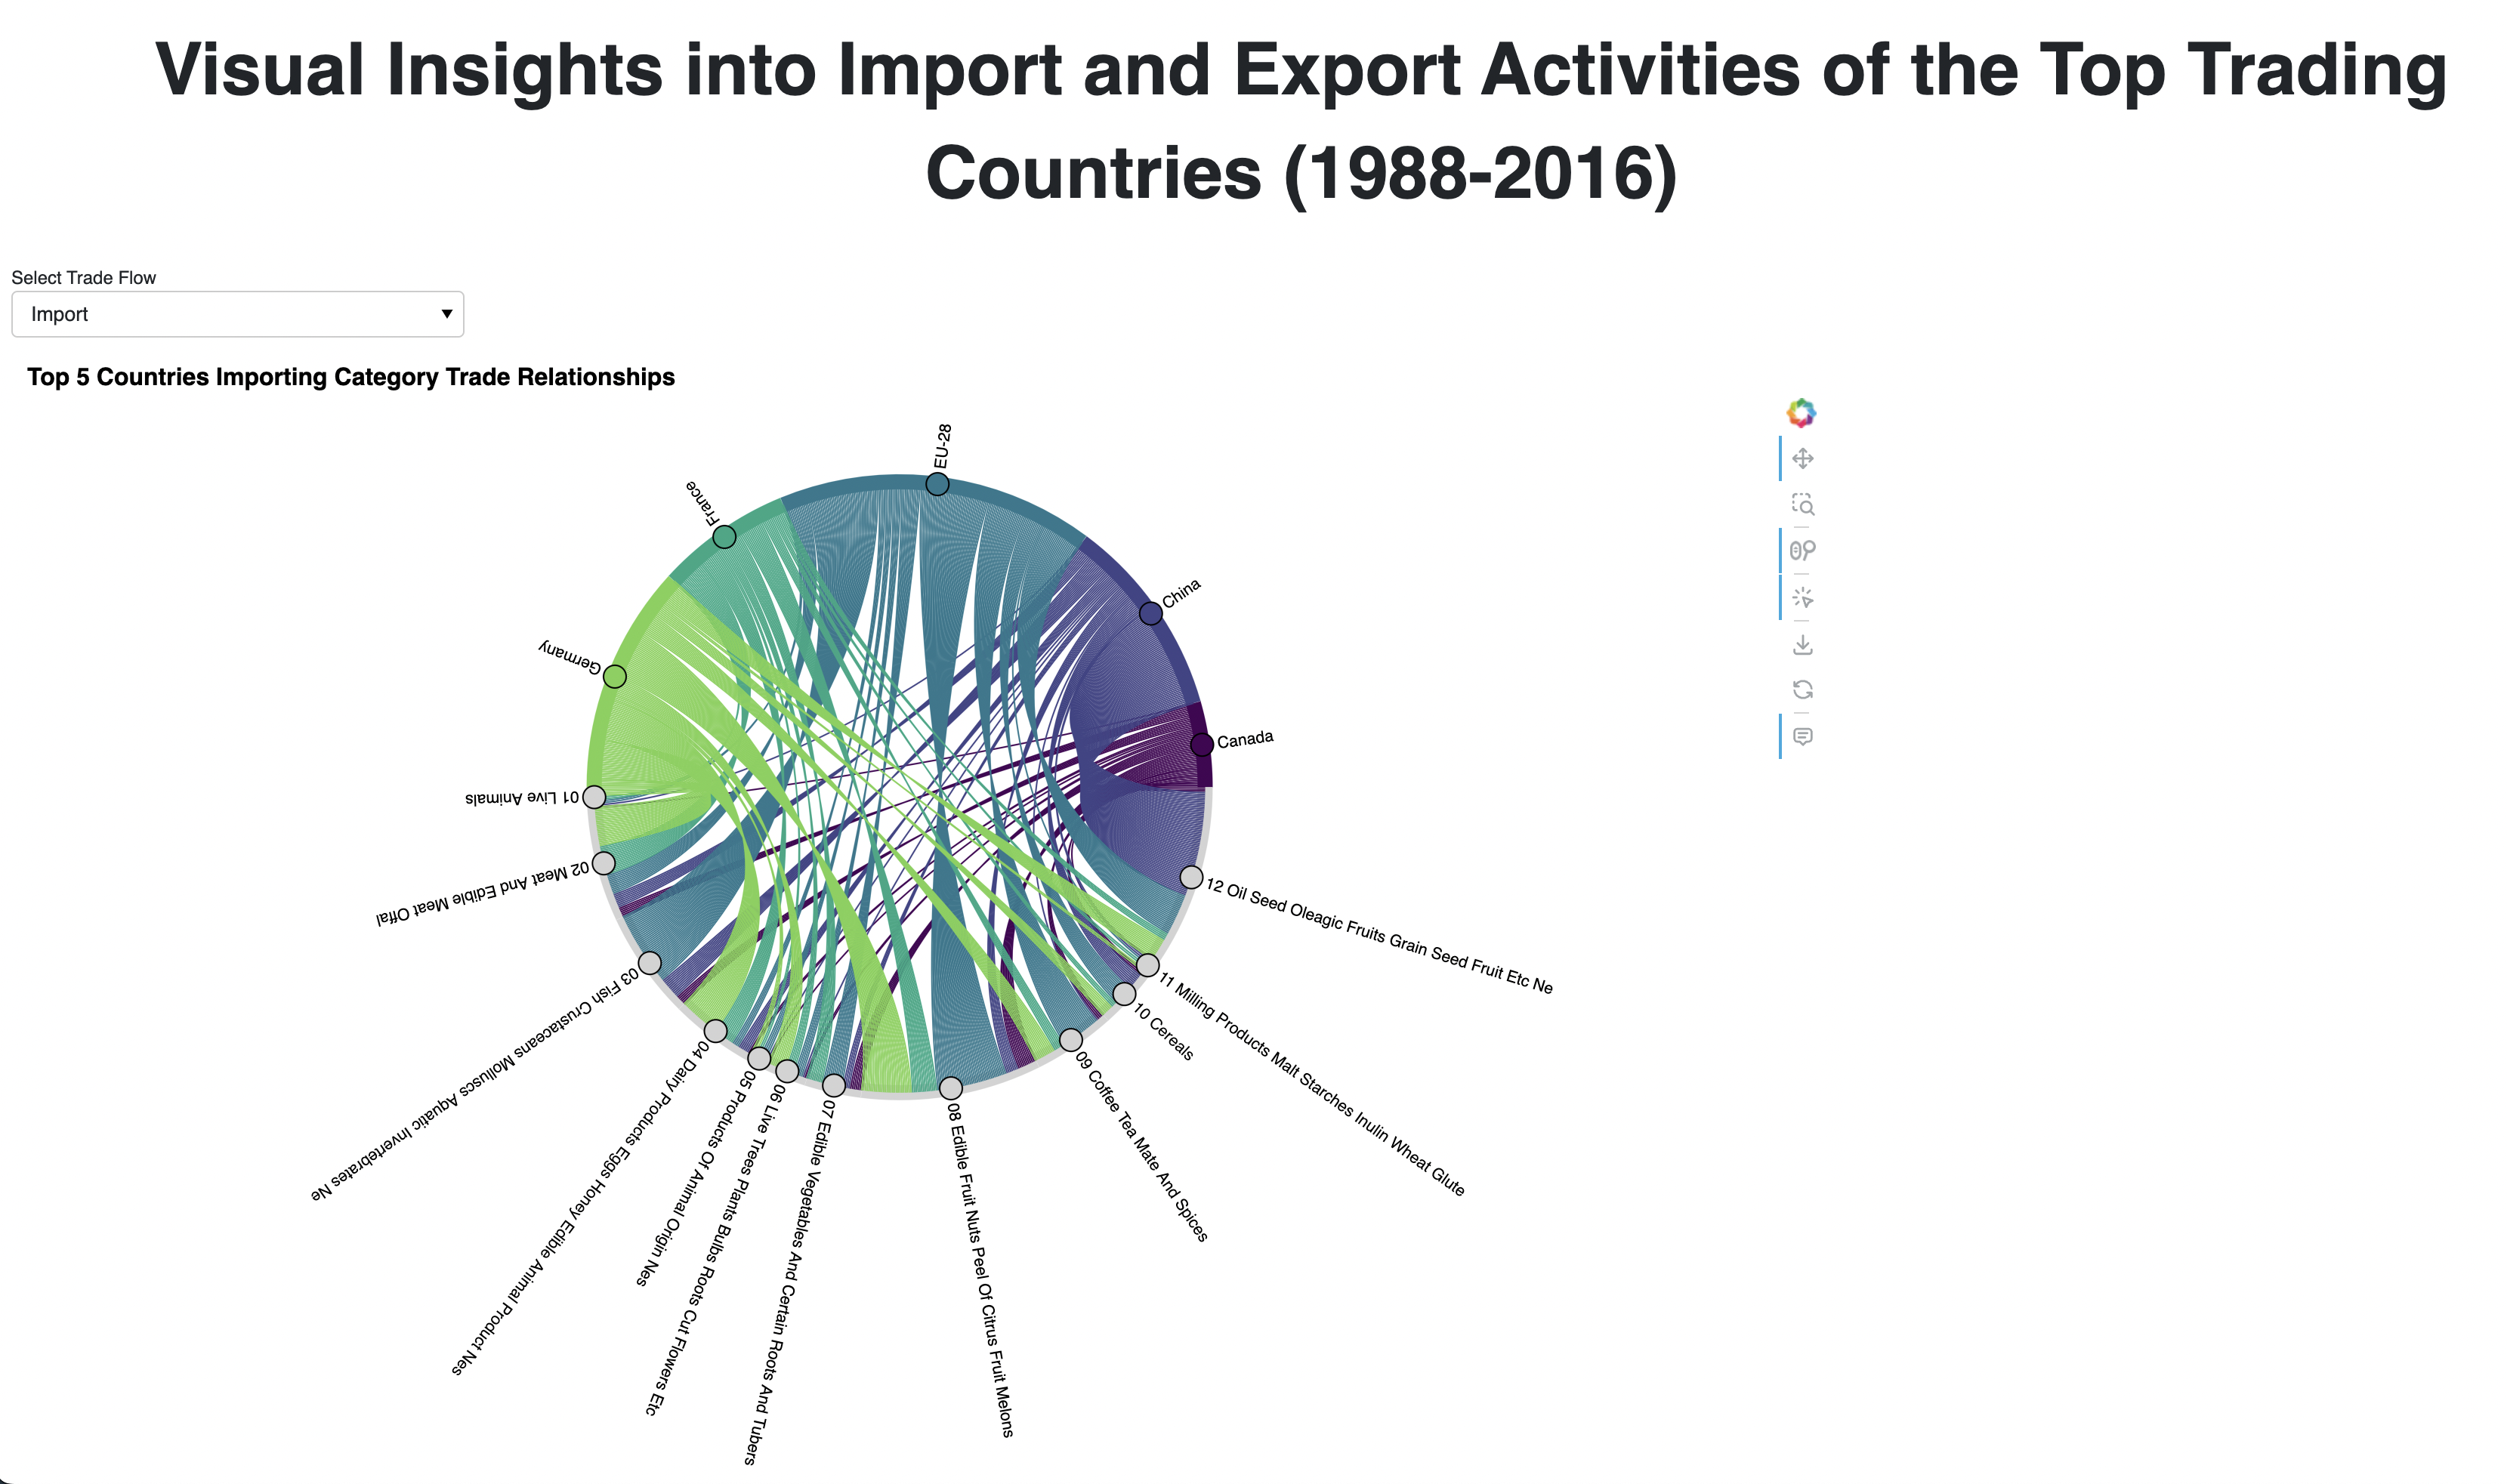
\includegraphics[width=1.003\textwidth]{st5442_assignment3/fig/Import.png}
    \caption{
        Visual Insights into Import Activities of the Top 5 Trading Countries (1988-2016)?
    }
    \label{fig:Import}
\end{figure}

Please be advised that the chord diagram has been zoomed out to encompass the entire title, filters, and all components of the visualization.

\begin{figure}[ht] 
    \centering
    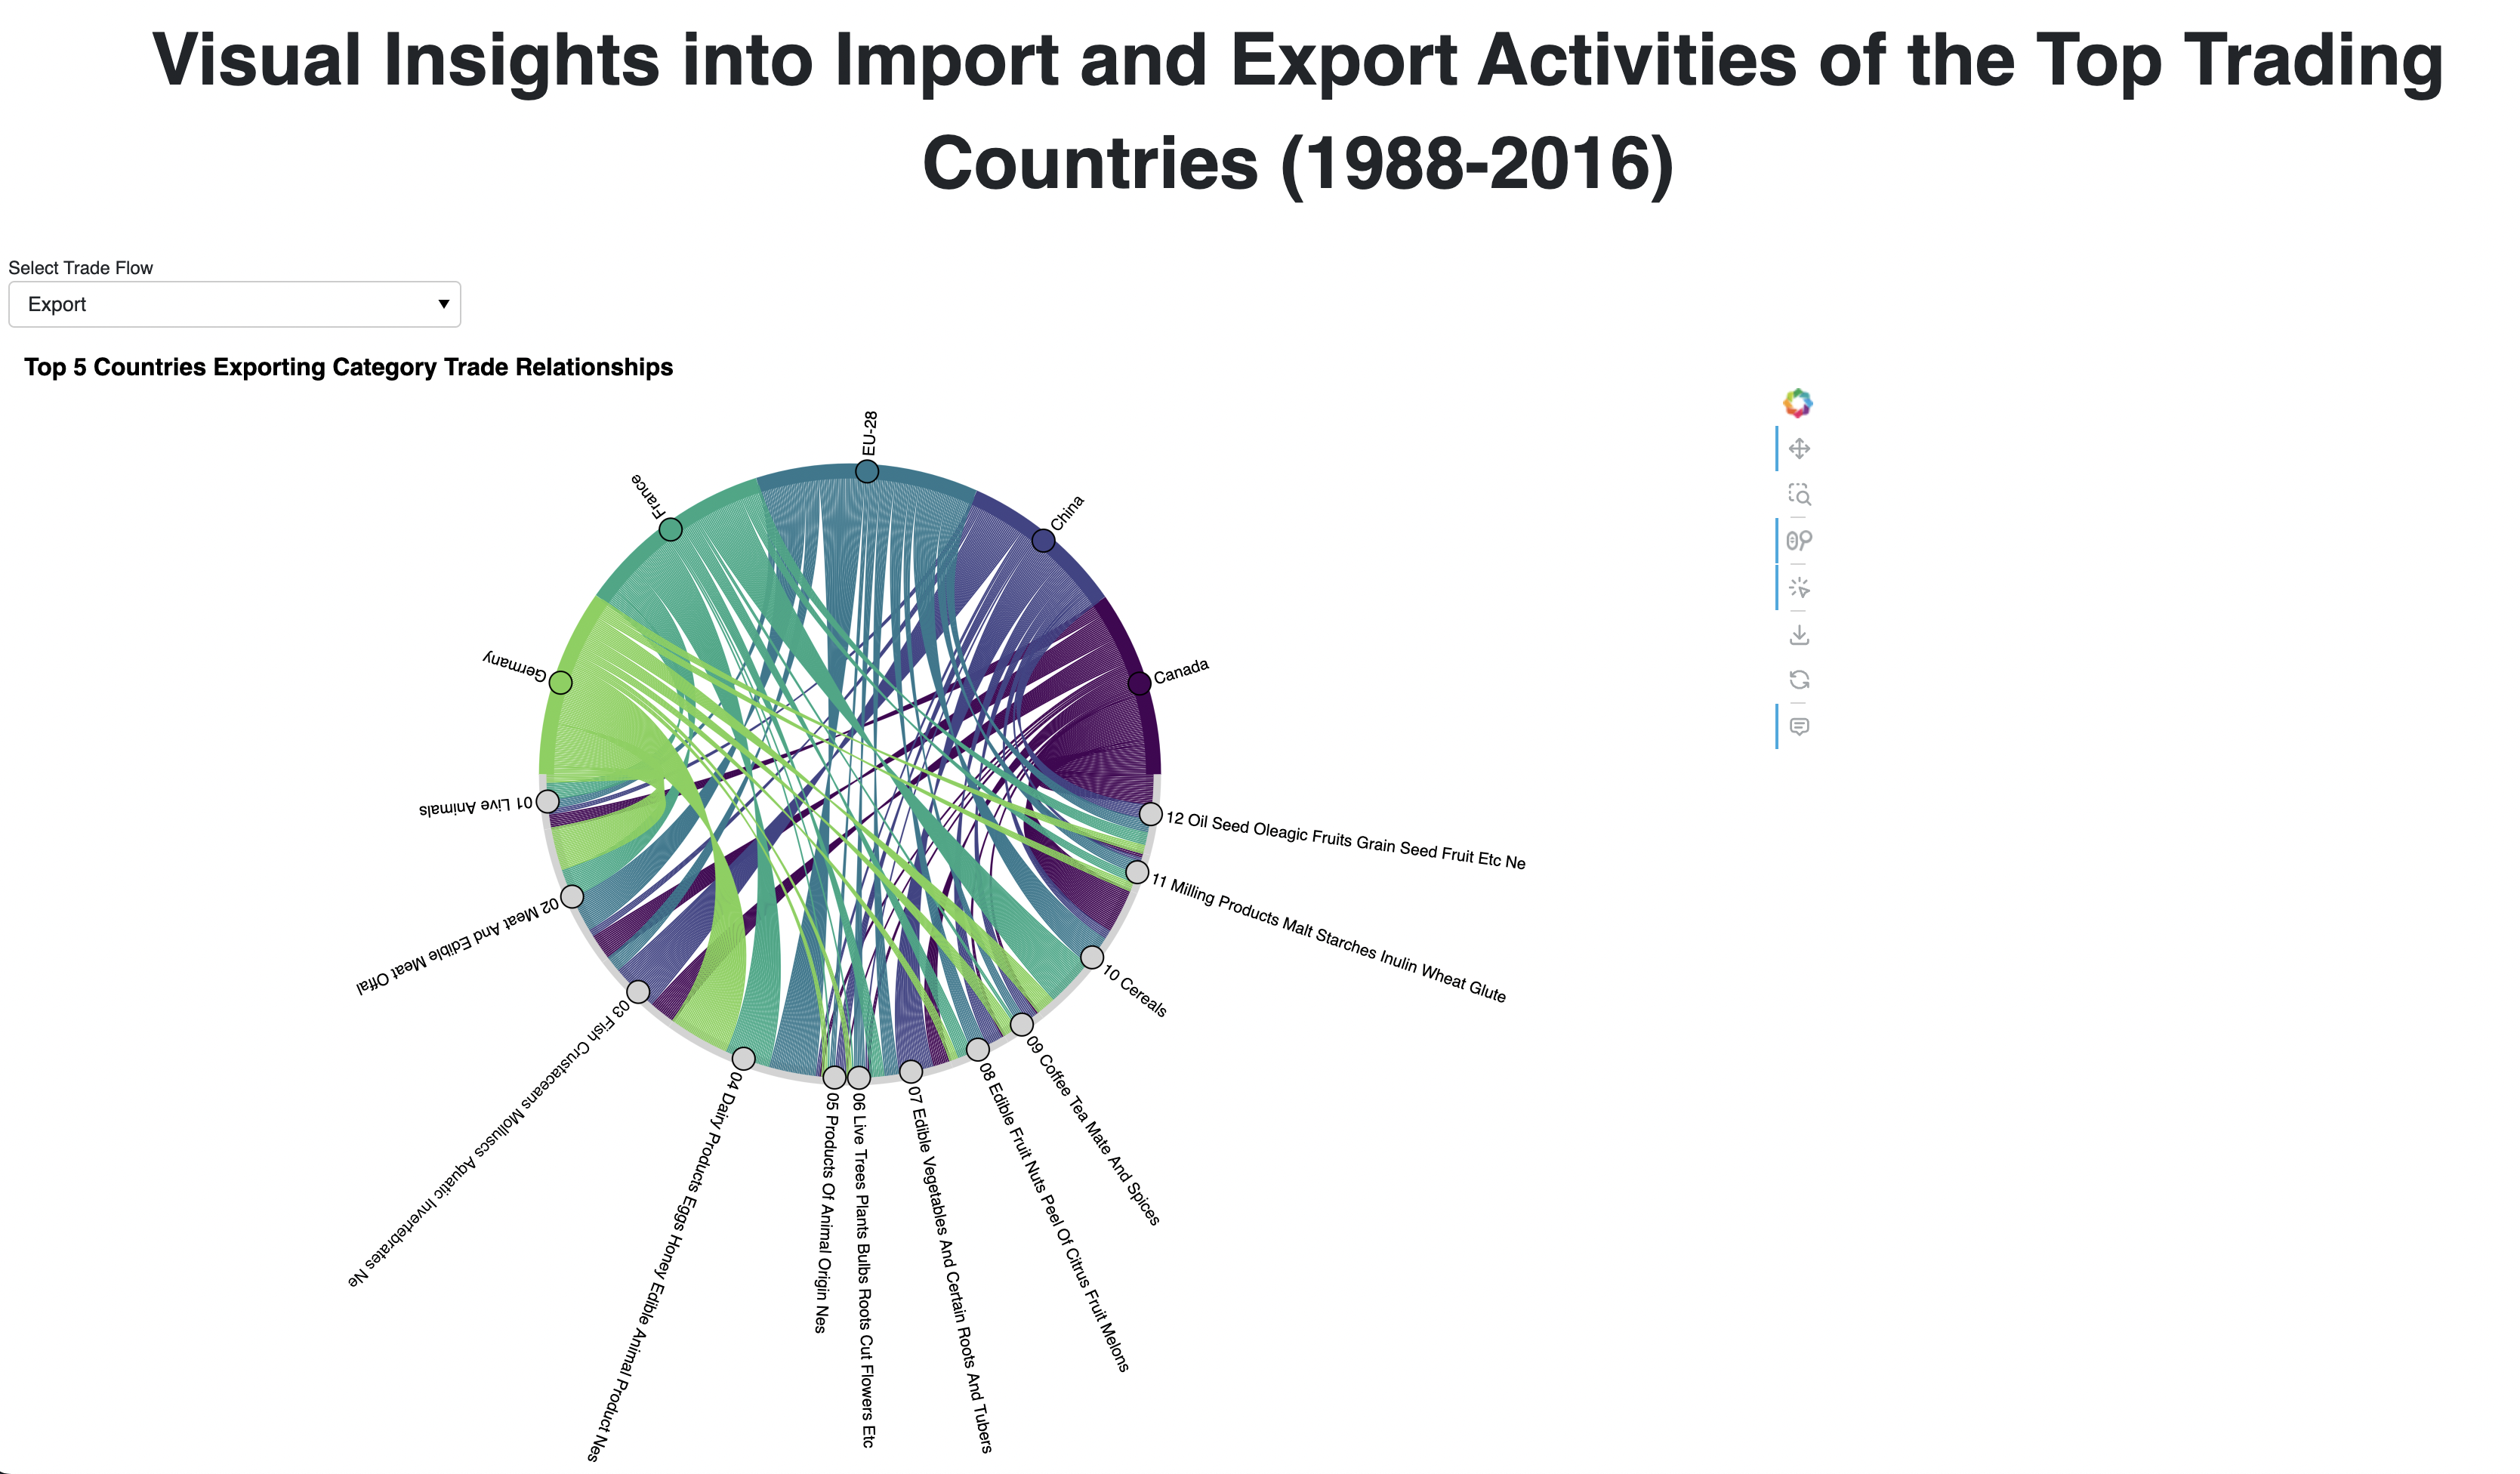
\includegraphics[width=1.003\textwidth]{st5442_assignment3/fig/Export.png}
    \caption{
        Visual Insights into Export Activities of the Top 5 Trading Countries (1988-2016)?
    }
    \label{fig:Export}
\end{figure}

\newpage

\section{Design Rationale}

\subsection{Data Preprocessing}
Before creating the visualization, the dataset was cleaned and processed. The initial steps included:
\begin{itemize}
    \item Loading the dataset from a CSV file containing trade statistics.
    \item Calculating the total trade value for each country to identify the top 5 countries by trade value.
    \item Filtering the dataset to focus on the selected countries and aggregating trade values based on categories and flow (import/export).
\end{itemize}

\subsection{Data Transformation}
The data was transformed to create a suitable format for the chord diagram:
\begin{itemize}
    \item Grouping the filtered data by country, category, and flow, aggregating trade values.
    \item Cleaning category names by replacing underscores with spaces and capitalizing them for better readability.
    \item Removing the "All Commodities" category to focus on specific trade relationships.
\end{itemize}

\subsection{Choice of Visualization}
A chord diagram\cite{chord} was selected for this visualization because of its efficacy in illustrating relationships among multiple entities in a clear and intuitive manner. This visualization method effectively represents trade connections between countries and various commodity categories, enabling users to quickly comprehend intricate interactions. The circular layout of the chord diagram facilitates an immediate understanding of the flow and magnitude of trade, making it particularly suitable for conveying complex data relationships in a compact format. 

\subsection{Color Encoding}
The color encoding for the visualization employs a Viridis colormap, recognized for its perceptually uniform color scale, which enhances visual accessibility. Each country is assigned a distinct color from this palette, while commodity categories are represented with a neutral hue. This method ensures clarity and interpretability, allowing users to easily differentiate between countries and categories while minimizing cognitive load. By utilizing the Viridis colormap, the visualization maintains an aesthetically pleasing and effective color scheme that supports data comprehension across various viewing conditions.

\subsection{Visual Encoding}
The visual encoding of the chord diagram includes:
\begin{itemize}
    \item \textbf{Nodes} are utilized to represent both countries and commodity categories, serving as the primary entities within the visualization.
    
    \item \textbf{Links} depict trade values between these nodes, with the thickness of each link correlating to the volume of trade, thereby providing an intuitive understanding of trade relationships.
    
    \item \textbf{Color assignment} for nodes is based on their classification (whether they represent a country or a commodity category), enhancing differentiation and aiding in the rapid identification of the relationships within the data. This structured visual encoding facilitates a clearer interpretation of the complex interactions present in the dataset.
\end{itemize}

\subsection{Additional Considerations}
Considerations included ensuring that the visualization is intuitive and user-friendly. The design emphasizes clarity and simplicity, avoiding unnecessary clutter to focus the viewer’s attention on the key insights.

\subsection{Interaction Techniques}
The primary interaction technique implemented is a dropdown menu that allows users to select between viewing import or export data. When a selection is made:
\begin{itemize}
    \item The chord diagram updates to reflect the selected trade flow, dynamically filtering the data and re-rendering the visualization.
    \item Additionally, when a user selects a specific country within the chord diagram, the edges connecting that country to its corresponding commodity categories are highlighted, while the edges to other countries become lighter. This visual effect draws attention to the selected country, helping users better concentrate on the trade relationships between that country and its respective import or export categories. This dual-layer of interactivity enhances user engagement and facilitates a deeper exploration of the trade data.
    \item Furthermore, the chord diagram supports zooming functionality, allowing users to magnify or reduce the view of the diagram. This capability is significant as it enables users to examine intricate details of the trade relationships at various scales, improving the accessibility of complex data patterns and enhancing the overall interpretability of the visualization. Users can zoom in to focus on specific nodes and links or zoom out to gain a broader overview of trade dynamics among multiple entities.
\end{itemize}

\subsection{Implementation}
The implementation was achieved using Python libraries such as HoloViews and Bokeh. The application is structured with Panel to create an interactive web-based interface, allowing users to explore the data in real-time. The layout includes a title, the dropdown for trade flow selection, and the chord diagram itself.

The dropdown functionality did not update the diagram when hosted as an HTML file, likely due to the specific interactivity requirements that are supported in Jupyter environments but not in static HTML exports. To resolve this issue and ensure the visualization works as intended, it was necessary to utilize the \texttt{.show()} method with \texttt{panel.serve()} to create a fully interactive dashboard. This approach allows the application to run a local server that correctly renders the interactive components. Since exporting to standalone HTML limits interactivity, the file \texttt{st5442\_assignment3.py} was served directly using the following terminal command:

\begin{lstlisting}[language=bash]
panel serve --show st5442_assignment3.py
\end{lstlisting}

It is important to ensure that the dataset is located in the same directory as the \texttt{.py} file when running this command. This setup allows users to engage with all the interactive features seamlessly.

\section{Insights}

\subsection{Import Flow}

\begin{itemize}
    \item \textbf{EU and China as Major Import Hubs:} The EU and China have large segments in the diagram, indicating they are prominent importers across various categories. This suggests a significant demand in these regions for diverse products, possibly due to their large populations and industrial needs.
    
    \item \textbf{Specialized Trade Categories:} Certain categories, like "Oil Seed Oleagic Fruits Grain" and "Edible Vegetables and Citrus," have thicker connections with specific countries, indicating that these goods are heavily imported by certain nations. For example, if a strong chord exists between Canada and "Oil Seed Oleagic Fruits Grain," it implies Canada is a primary importer of this product category.
\end{itemize}

\subsection{Export Flow}

\begin{itemize}
    \item \textbf{EU and China as Key Exporters Across Multiple Categories:} Both the EU and China have substantial segments with multiple connections to various trade categories, indicating that they are primary exporters across diverse sectors. This diversity suggests a strong industrial base, allowing these regions to produce and export a wide range of goods.
    
    \item \textbf{Product Specialization for Specific Countries:} Certain countries have strong connections to particular categories, which could imply specialization. For example, if the U.S. has a thick chord connected to "Milling Products, Malt, Starches, Inulin, Wheat Gluten," it may indicate that the U.S. specializes in exporting this category, possibly due to its extensive agricultural sector that supports grain and wheat production.
\end{itemize}



\section{Strengths and Weaknesses}

\subsection{Strengths}
\begin{itemize}
    \item \textbf{Clarity:} The chord diagram effectively communicates trade relationships, making complex data more comprehensible.
    \item \textbf{Interactivity:} The dropdown feature enhances user engagement, allowing for targeted exploration of the data.
    \item \textbf{Visual Appeal:} The color scheme and layout are visually appealing and easy to navigate.
\end{itemize}

\subsection{Weaknesses}
\begin{itemize}
    \item \textbf{Data Limitations:} The focus on only the top 5 countries may overlook significant trade relationships involving other countries.
    \item \textbf{Scalability:} As the number of countries or categories increases, the chord diagram may become cluttered and harder to interpret.
    \item \textbf{Dependency on Filtering:} If the filtered dataset yields no results for the selected trade flow, users may encounter a lack of visual output, which could be confusing.
\end{itemize}



\section{Conclusion}

In conclusion, this project successfully demonstrated the potential of interactive visualizations to elucidate the complex trade relationships between countries and commodity categories. By employing a chord diagram, the visualization effectively highlights the import and export activities of the top five trading nations, allowing users to explore data dynamically through the dropdown menu. The interactivity enhances user engagement, facilitating a deeper understanding of the data by allowing for the selective display of trade flows.

The choice to implement the visualization in a \texttt{.py} file, served locally via \texttt{panel.serve()}, was crucial for maintaining the interactivity of the dashboard. This method ensured that users could fully engage with the visualization without the limitations imposed by static HTML exports. Furthermore, the visual design choices and interaction techniques were carefully crafted to provide an intuitive and informative user experience.

Overall, this project not only highlights the intricate connections in global trade but also serves as a foundation for future explorations of interactive data visualization techniques.

\newpage



\begin{refcontext}[sorting=nyt]
\printbibliography
\end{refcontext}

\end{document}

